\documentclass[a4paper,titlepage]{article}
\usepackage[utf8]{inputenc}
\usepackage{a4wide}
\usepackage[T1]{fontenc}
\usepackage{times}
\usepackage{color}
\usepackage[dvipsnames]{xcolor}
\usepackage{fancyhdr} %% Package to create a header on each page.
\usepackage{lastpage} %% Used for "Page X of Y" in the header.
\usepackage{refcount}
\usepackage{fp}
\newcommand{\pagerefprev}[1]{
	 \FPeval{\result}{clip(\getpagerefnumber{#1}-1)}
	 \result
}

% German
\usepackage[ngerman]{babel}
% English
%\usepackage[english]{babel}

\usepackage[round,authoryear]{natbib}
\usepackage{amsmath,amssymb,amsthm}
\usepackage[hyphens]{url}
\usepackage[colorlinks=true, urlcolor=blue, linkcolor=black ]{hyperref}
\usepackage{graphicx}
\usepackage{wrapfig}
\usepackage{subcaption}
\usepackage{float}
\usepackage[font=small,labelfont=bf]{caption}
\usepackage[title]{appendix}
\usepackage{enumitem}

\usepackage{scrextend}
\deffootnote[1em]{1em}{1em}{\textsuperscript{\makebox[1em][l]{\thefootnotemark}}} %no indent of footnote

%inline code formating
\usepackage{xcolor}
\definecolor{codeColor}{gray}{0.1}
\newcommand{\ilc}[1]{\textcolor{codeColor}{\texttt{#1}}}

\fancyhf{}
%% Left side of header
\lhead{\titleName}
%% Height of header
%\usepackage[top=2.5cm,bottom=2.5cm, left = 2cm, right=2cm]{geometry}
%% Right side of footer
\rhead{Seite \thepage\ von\pagerefprev{appendixPage}}
%% Page style that uses the header
\pagestyle{fancy}

\newcommand{\titleName}{Multi Device Feed}
\renewcommand{\thefigure}{\thesection.\arabic{figure}}

\setlength{\parindent}{0pt}
\usepackage[parfill]{parskip}
\setlength{\parskip}{0.8em}

\begin{document}

% Titelseite
% - - - - - - - - - - - - - - - - - - - - - - - 

\begin{titlepage}
	\begin{tabular}{@{}ll}
		Kurs: &\indent Introduction to Internet and Security (IaS), Frühjahrsemester 2021  \\
		Dozenten: &\indent Prof. Dr. Christian Tschudin  \\
		Datum: &\indent 18. Juli 2021
	\end{tabular}
	\vspace*{1cm}   
	\begin{center}
		\large
		{\color{NavyBlue}{Projekt Report}} \\	
		\vspace*{1cm}   
	        \Huge
	        {\color{NavyBlue}{BACnet: \\ \titleName}}\\
	        \Large
        	\vspace*{1cm}   
	        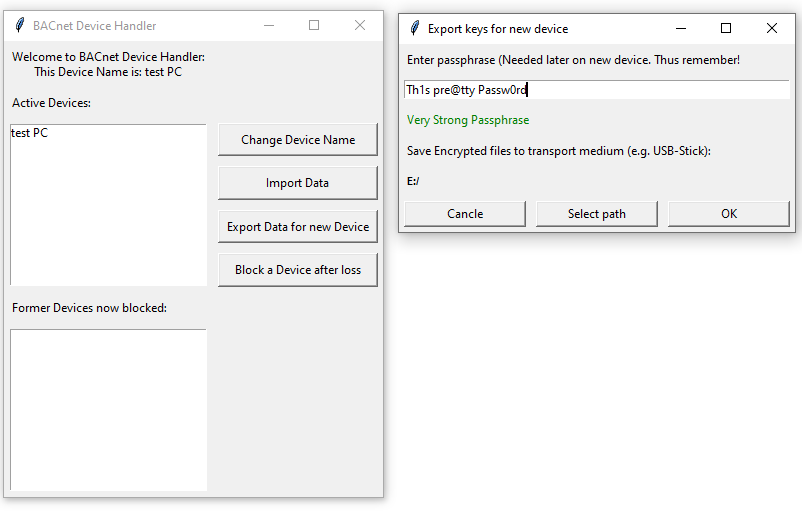
\includegraphics[width=0.75\textwidth]{figures/UIexport}  
		\vfill
	        \normalsize
		\begin{tabular}{@{}ll}
			Gruppe 10 \\
			Matthias Müller &\indent \href{mailto:matthias01.mueller@stud.unibas.ch}{matthias01.mueller@stud.unibas.ch}  \\
			Patrick Steiner &\indent \href{mailto:pa.steiner@stud.unibas.ch}{pa.steiner@stud.unibas.ch}  \\
			Reto Krummenacher &\indent \href{mailto:reto.krummenacher@unibas.ch}{reto.krummenacher@unibas.ch}
		\end{tabular}
	\end{center}  
\end{titlepage}

% Report
% - - - - - - - - - - - - - - - - - - - - - - - 
\clearpage
\setcounter{page}{1}


\section{Einleitung}

Das BACnet ist eine dezentralisiertes Netzwerk, welche ohne das Internet und dessen gängige Protokolle (IP, TCP) die Kommunikation zwischen Teilnehmern ermöglicht. Die einfachste Art der Informationsübertagung ist die Übergabe von USB-Sticks mit den gewünschten Daten der Applikationen. Jede Applikation erstellt ihre eigenen Feeds mit einem privaten und öffentlichen Schlüssel. Eine Feed kann als erweiterbare aber nicht veränderbare verkettete Liste betrachtet werden. Anhand des öffentlichen Schlüssels sind die einzelnen Feeds unterscheidbar. Ein Nutzer im BACnet wird anhand eines sogenannten Master-Feeds\footnote{Dies basiert auf Arbeiten aus dem Frühjahrsemester 2020: \\ \url{https://github.com/cn-uofbasel/BACnet/tree/master/20-fs-ias-lec/groups/14-feedCtrl} \\ (letzter Aufruf 11.07.2021)} eindeutig identifiziert.

Bisher war es einem Teilnehmer im BACnet nicht möglich, die gleiche Applikation von verschiedenen Geräten zu bedienen. Dazu müssen die Privaten Schlüssel der Feeds geteilt werden, damit der gleiche Benutzer auf einem anderen Gerät die selben Feeds erweitern kann. Damit besteht die Gefahr von Kollisionen. Ein Nutzer schreibt von Gerät A und B gleichzeitig in einen Chat. Das dezentrale BACnet hat keine automatische Synchronisation, sprich die Daten von Gerät A werden nicht sofort auf das Gerät B übertragen. Für den Chatpartner müssen die unterschiedlichen Einträge von Gerät A und B zusammengefügt werden. Vor dem Hintergrund der BACnet Prämisse von nicht veränderbaren Feeds ist dies nicht möglich. Eine Lösung sind virtuelle Feeds.

Ziel dieses Begleitprojekts im Rahmen der Vorlesung `Internet and Security' ist das Entwickeln eines Systems virtueller Feeds für das BACnet sowie einer Möglichkeit der Geräteverwaltung für den Benutzer. Dies aufbauend auf den Arbeiten des Frühjahrsemester 2020. Der vorliegende Bericht erläutert die erarbeiteten Lösungen und beschreibt die erstellten Python-Module \footnote{Sämtlicher Code findet sich unter: \\ \url{https://github.com/cn-uofbasel/BACnet}} konzeptionell. In einem ersten Teil werden die virtuellen Feeds behandelt, während die Geräteverwaltung in einem zweiten Teil besprochen wird. Abschluss bildet die kritische Würdigung der Arbeiten. Im Anhang finden sich sämtliche Abbildungen sowie die Liste verwendeter Python-libraries.


\section{Virtuelle Feeds}

\textcolor{red}{bitte erwähnen das virtuelle Feeds gebraucht werden, dies ist die Einleitung zum teil zwei}





\section{Geräteverwaltung}
Zu den Aufgaben der Geräteverwaltung zählt einerseits das Verteilen von privaten Schlüssel auf weitere Geräte eines Nutzers sowie das Gerätemanagement generell.  Die Klassen und Methoden stellen die Funktionalität sowie eine GUI bereit.

\subsection{Funktionalität}
Die gesamte Funktionalität ist in \ilc{uiFunctions.py} implementiert. 

\subsubsection*{Schlüsselverteilung}
Wie im vorangehenden Kapitel erläutert, benötigen virtuelle Feeds einen gemeinsamen geheimen Schlüssel. Dieser muss auf allen Geräten identisch sein und daher geteilt werden können, ohne für Dritte lesbar zu sein . Daraus folgt, dass Geräte A und B einen gemeinsamen privaten Schlüssel benötigen, um den virtuellen Feed Schlüssel chiffrieren und dechiffrieren zu können.  Das teilen von privaten Schlüssel ist unter dem Begriff `Key exchange problem' bekannt. Dies kann mittels Verwendung eines asymmetrischen Schlüsselpaars umgangen werden. Zu sendende Informationen werden mit dem öffentlichen Schlüssel des Empfängers codiert. Nur mit dem privaten Schlüssel des Empfängers ist eine Decodieren möglich. Im vorliegenden Fall ist dies nicht praktikabel, da das Erstellen eines asymmetrischen Schlüsselpaars den Austausch der dazu notwendigen Informationen benötigt. Im dezentralen BACnet erfordert dies ein mehrmaliges hin und her reichen eines USB-Sticks. Aus diesem Grund haben wir uns für eine symmetrischen Verschlüsselungsverfahren mit einem gemeinsamen privaten Schlüssel entschieden. 

Unser Lösungsansatz ist, dass der gemeinsame private Schlüssel gar nicht geteilt, sonder auf jedem Gerät individuell erstellt wird. Dazu verwenden wird den gleichen Algorithmus auf beiden Geräten zusammen mit einem vom Benutzer bereitgestellten Password. Dieses Verfahren ist als `password based key derivation' bekannten und von der IETF\footnote{Internet Engineering Task Force, RFC 8018, Password-Based Cryptography Specification Version 2.1\\ \url{https://datatracker.ietf.org/doc/html/rfc8018\#appendix-A.2} \\ (letzter Aufruf 11.07.2021)} empfohlen. Die Daten, hier die geheime Feed Schlüssel eines Benutzers, werden mit dem passwortbasierten Schlüssel auf Gerät A chiffriert und auf einem Transportmedium gespeichert. Nur mit dem Passwort ist ein Dechiffrieren auf Gerät B möglich.

Um die Stärke des eingegebenen Passworts zu bewerten, wird dessen Entropie berechnet. Die Entropie wird durch die Lange und die Menge der möglichen Zeichen bestimmt.\footnote{Berechnung der Entropie im Detail: \\ \url{https://www.omnicalculator.com/other/password-entropy} \\ (letzer Aufruf 9.7.2021)} Je höher der Wert, desto mehr Kombinationen ($2^{Entropie}$) gibt es. Entsprechenden länger dauert ein Brut-Force erraten des Passworts.

\subsubsection*{Geräte hinzufügen, benennen und blockieren}
Neben der Schlüsselweitergabe ist das Benennen und Blockieren der registrierten Geräte von Bedeutung. Jedes Gerät verfügt über eine Identifikationsnummer und einen privaten Schlüssel. Beides wird beim erstmaligen Ausführen erstellt und lokal gespeichert. Gleichzeitig wird ein provisorischer Benutzername zugeordnet. Anhand der eindeutigen unveränderlichen Nummer kann ein Gerät identifiziert werden, während der Name selbst vom Benutzer nach Wunsch geändert werden kann. Ein Gerät kennt zwei Zustände, aktiv und blockiert. Jedes neu registrierte Gerät wird zunächst als aktiv gekennzeichnet. Die gesamten Informationen werden lokal gespeichert und simultan zur Schlüsselverteilung ebenfalls auf das Transportmedium übertragen. Über die Zeit entsteht ein Verzeichnis aller Geräte eines Benutzers.

Ein wesentliches Problem im Zusammenhang mit verschiedenen Geräten ist ein möglicher Verlust eines solchen. Darauf enthaltene Informationen sind in jedem Fall verloren. Noch vorhandenen historischen Meldungen des abhanden gekommen Geräts können weiterhin verwendet werden, falls dessen Identifikationsnummer bekannt bleibt. Auf Basis dieser Tatsache haben wir uns dazu entschlossen, keine Geräte zu löschen, sondern diese nur zu blockieren. Die Nummer verbleibt im Geräteverzeichnis.

\subsection{GUI}
Die GUI wurde mit \ilc{tkinter} erstellt und ist in \ilc{ui.py} implementiert. Die graphische Benutzeroberfläche bildet denn Einstiegspunkt der Geräteverwaltung. Beim erstmaligen Ausführen auf einem Gerät wird automatisch eine Geräteschlüssel und ein Gerätename kreiert. Das Hauptfenster ermöglicht dem Benutzer die Funktionalitäten der Geräteverwaltung per Klick auszuführen. Darunter das Exportieren und Importieren der Feed-Schlüssel. Der jeweiligen Button öffnet ein Dialog-Box, worin der Nutzer die benötigten Informationen wie Pfad oder Passwort eingeben kann. Abbildung \ref{fig:UI} zeigt das Hauptfenster zusammen mit dem geöffneten Exportdialog. Letzterer enthält einen Hinweis zur Stärke des eingegebenen Passworts. Das Angezeigte Geräteverzeichnis bietet die Optionen, Geräte zu blockieren. Ein Umbenennen ist nur für das aktuelle in Gebrauch befindliche Gerät erlaubt.

\section{Fazit}
Die Geräteverwaltung bietet die geforderte Funktionalität sowie eine benutzerfreundliche GUI zur chiffrierten Übertragung privater Schlüssel zwischen Geräten. Ebenfalls ....

\textcolor{red}{Positives Fazit zu eurem Teil}

Zusammenfassend lässt sich sagen, dass die im Verlauf dieses Projekts festgelegten Anforderungen mehrheitlich erfüllt wurden. Nicht erreicht wurde der Aufbau unserer Lösung für virtuelle Feeds auf das im Frühjahrsemester 2021 von der BACnet Core Gruppe entwickelte System. Dies ist der Tatsache geschuldet, dass den dortigen Neuerungen von uns zu spät Beachtung geschenkt wurde. In einer Gesamtbetrachtung überwiegen jedoch die positiven Punkte, weshalb wir dieses Begleitprojekt als Erfolg bewerten.


\clearpage
\pagestyle{empty}
\fancyhf{}
\lhead{\titleName}
\pagestyle{fancy}
\lhead{\titleName}
\label{appendixPage} % needed to calculate page of page, as Appendix has no page numbers

% Referenzen
% - - - - - - - - - - - - - - - - - - - - - - - 

%\begin{itemize}
%	\item Fitzgerald, Scott und Shiloh, Michael (Hrg.), The Arduino Projects Book, 2015. (dem Arduino Starterkit beiliegend).
%\end{itemize}

% Anhang
% - - - - - - - - - - - - - - - - - - - - - - - 

\clearpage
\section*{Anhang}
    	\renewcommand\thesubsection{Anhang \arabic{subsection}} %new title of section
   	\renewcommand\thesubsubsection{\arabic{subsection}.\arabic{subsubsection}} %new title of subsubsection
   	\setcounter{figure}{0} 
   	  
	\subsection{Python libraries} \label{libraries} % label um zu referencieren \ref{labelname}
		\begin{itemize}
			\item \ilc{cryptography} \\
				\url{https://cryptography.io/en/latest/} (letzter Aufruf 11.07.2021)
				\begin{itemize}[label={}]
				\item \ilc{.hazmat.primitives.kdf.pbkdf2.PBKDF2HMAC} \\
					Erstellen eines Key auf Basis eines Passworts
				\item \ilc{.hazmat.primitives.ciphers.aead.AESGCM} \\
					Verschlüsselung mittels AES und GCM mittels Key
				\item \ilc{.hazmat.primitives.hashes}\\
					Enthält den Algorithmus SHA256
				\item \ilc{.exceptions.InvalidTag}\\
					Exception beim Entschlüssel mit falschem Passwort 
				\end{itemize}
			\item \ilc{getpass} \\
				Bestimmung des Benutzernamens auf dem Betriebssystem
			\item \ilc{json} \\
				Library für den Umgang mit JSON-Dateien
			\item \ilc{math} \\
				Mathematische Operationen
			\item \ilc{os} \\
				Pfad und Datei Methoden
			\item \ilc{re} \\
				Verwendung von regulären Ausdrücken	
			\item \ilc{secrets} \\
				Erstellen von Test-Keys für das Testing
			\item \ilc{shutil} \\
				Kopieren von Dateien
			\item \ilc{tkinter} \\
				Erstellen einer GUI				
			\item \ilc{unittest} \\
				Wird in der Klasse \ilc{TestMethods} verwendet. Diese enthält Funktionstest des Device Handlers.
		\end{itemize}
		
\newpage

	\subsection{Abbildungen}
		\subsubsection{GUI} 	\label{fig:UI}
		\begin{figure}[H] %this figure will be at the right
			\centering
			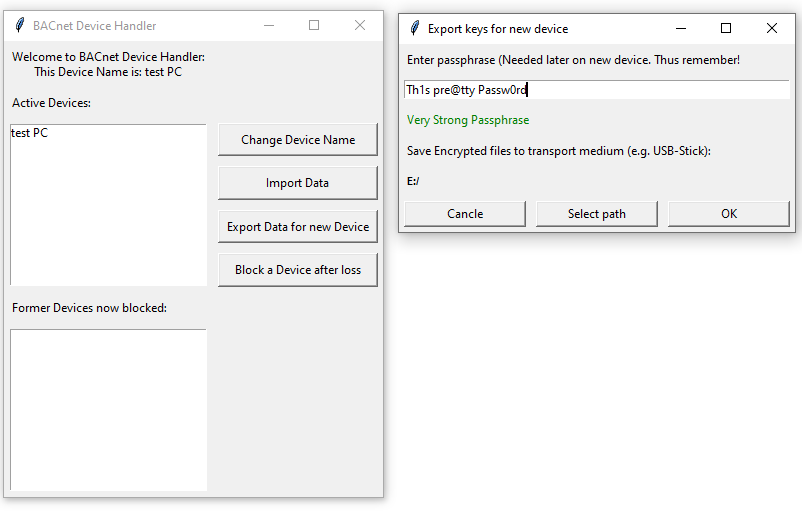
\includegraphics[width=1\textwidth]{figures/UIexport}
			\caption*{Das Hauptfenster und der geöffnete Exportdialog, welcher ein Hinweis zur Passwortstärke enthält.}
		\end{figure}
		
		\subsubsection{}
		
\end{document}

